\chapter{Optimalisatie}
\label{opt}

De bedoeling van de optimalisatie is het vergroten van het percentage nuttige connecties. Met basis LCF's werd er enkel in de tijd gefilterd waardoor ook connecties van ontoegankelijke stopplaatsen werden teruggeven. De optimalisatietechnieken die in dit hoofdstuk besproken worden, zullen dit probleem proberen oplossen met behulp van geofiltering.

\section{Geofiltering}

Het CSA-algoritme bouwt met de binnenkomende connecties een minimale overspannende boom. Dit kan visueel voorgesteld worden als een cirkel rondom het vertrekpunt van de query. Het idee van geofiltering bij Linked Connections is om enkel connecties gesorteerd in de tijd �n afstand van het vertrekpunt terug te geven. Een extra filter betekent extra HTTP parameter(s).

\subsection{Geoparameter}
Een eerste inspiratie was om connecties onder te verdelen zoals kaarten als Open Street Maps werken. Hierbij wordt er met \textit{tiles} gewerkt. Een \textit{tile} is een rechthoekig stuk van een kaart die op basis van drie parameters kan ge\"identificeerd worden: het x- en y-co\"ordinaat en een \textit{zoomlevel} z. Bij statische data zoals kaarten is dit zeer handig, omdat deze stukjes cachebaar zijn. Bij transportdata moet er ook rekening gehouden worden met tijd, waardoor zo'n systeem niet haalbaar is.

Resources zijn pas cachebaar als er een beperkte set van URL's zijn. Aangezien elke publieke transportmaatschappij een beperkte set stops heeft, wordt er geopteerd om het vertrekpunt van een query toe te voegen als extra HTTP parameter. Listing \ref{nieuwe-interface}) toont deze nieuwe interface. Connecties die in de buurt van de vertrekstop liggen, hebben zeker initieel een grotere kans om gebruikt te worden. In volgende subsectie bespreken we de criteria om connecties terug te geven. 

\begin{lstlisting}[label=interface-optimalisatie,caption=Interface LDF met optimalisatie]
http://example.org?departureTime={...}&departureStop={...}
\label(label:nieuwe-interface)
\end{lstlisting}

\subsection{Criteria}
In eerste instantie moeten we een "straal"-definitie bepalen. Hiervoor zijn er twee mogelijkheden:

\begin{itemize}
\item De straal tussen de vertrekstop en een stop $s$ is het minimaal aantal connecties nodig om deze te bereiken. Een straal van grootte een stemt overeen met stops die met een connectie bereikt kunnen worden. Een straal van grootte twee is een stop waarvoor twee connecties nodig zijn enzovoort. Connecties worden als het ware \textit{gejoint} aan elkaar.
\item Het minimum aantal overstappen (Engels: \textit{transfers}) wordt als straal van een stop genomen. Dit geeft extra interessante mogelijkheden zoals Pareto-optimale routes bepalen op basis van snelste aankomsttijd �n maximaal aantal overstappen. Dit idee wordt ook bij RAPTOR (\ref{raptor}) gebruikt. Voortaan zullen we de letter $K$ gebruiken voor het minimum aantal overstappen.
\end{itemize}

Deze masterproef maakt gebruik van het aantal overstappen. 

Twee nieuwe termen zullen regelmatig gebruikt worden:
\begin{itemize}
\item \textit{direct bereikbare stop}: dit is een stop dat zonder overstappen bereikbaar is vanuit de vertrekstop. In GTFS termen betekent dit dat de snelste route slecht uit een trip kan bestaan.
\item \textit{indirect bereikbare stop}: dit is een stop die minstens K overstappen vereist vanuit de vertrekstop.
\item \textit{buur}: dit is een stop die direct of indirect bereikbaar is.
\end{itemize}

Een andere belangrijke criteria om geoptimaliseerd connecties terug te geven is dat er geen connecties teruggeven mogen worden van buren die theoretisch gezien nog niet bereikbaar zijn. Voor elke buur is een bepaalde \textit{minimale tijd} nodig om deze te bereiken.

Kortom, voor elke stop moet zijn buren bepaald worden samen met informatie over het minimaal aantal overstappen en minimale tijd om deze te bereiken. Hiervoor wordt er een extra voorbewerkingsfase toegevoegd en wordt er een extra \textit{feature} aan het connectiegenerator script toegevoegd.

\subsection{Direct bereikbare stops}

Connecties worden gegenereerd uit een reeks stoptijden van dezelfde trip. Dit is informatie die gebruikt kan worden om direct bereikbare stops te berekenen. Zo'n reeks stelt een aantal paren stops voor met een bepaalde tijd die nodig is in die trip. Tijdens het genereren van connecties wordt voor elke stop een minimale overspannende boom bijgehouden met als knopen rechtstreeks bereikbare stops en als verbindingen de minimale tijd. Nadat de connecties gegenereerd zijn wordt deze informatie weggeschreven naar een CSV-bestand zodat we dit kunnen hergebruiken om buren mee te berekenen.

\subsection{Buren}

Het berekenen van buren houdt het vinden van niet-direct bereikbare stops voor elk stop in. Een indirect bereikbare stop van $s$ met minimum aantal overstappen $K=1$ is een direct bereikbare stop van een direct bereikbare stop van $s$ die niet direct bereikbaar is bij $s$ zelf. Als er $n$ stops zijn in een dataset, moeten er $n*n$ afstanden berekend worden. Dit zou gemakkelijk met Floyd-Warshall kunnen, maar bij grote netwerken zoals bij De Lijn is er een probleem met geheugen. De Lijn heeft namelijk afgerond 35000 stopplaatsen waardoor een matrix van 35000 x 350000 in het geheugen moet gehouden worden. Om dit toch te kunnen berekenen, maken we gebruik van een algoritme die gebaseerd is op Dijkstra. Pseudocode hiervan is te vinden in \ref{mob-stop}. Er kan ingesteld worden tot hoeveel overstappen er verder gezocht moet worden. Het algoritme maakt gebruik van een wachtrij van stops die nog bekeken moeten worden. Elke stap probeert de minimale tijdsafstand en/of aantal overstappen te minimaliseren van een buur van een stop. Het object dat bekomen wordt voor een bepaalde stop staat afgebeeld in listing \ref{serverstopdata}. Dit wordt weggeschreven naar een aparte buren-tabel op een LC server.

\begin{lstlisting}[label=serverstopdata,caption=Data over stop serverside]
{
	stop_id : 123,
	aantal_direct_bereikbare_stops: X,
	// andere metadata over de stop
	buren: [
		{
			stop_id: 253,
			minimaleTijdsAfstand: 1800, // seconden
			K: 2
		}, {
		...
		}
	]
}
\end{lstlisting}

\begin{algorithm}
  \caption{Berekenen van Minimale Overspannende Boom van burenstops voor een GTFS stops.txt. $T$ is het maximaal aantal overstappen waarmee rekening gehouden wordt.}
  \label{mob-stop}
  \begin{algorithmic}
  \State K $\leftarrow$ natuurlijk getal
  \For { elke stop $s$ in stops.txt }
  \Statex // Initialisatie
    \State var mob = \{\};
    \State var wachtrij = []; // nog te bezoeken stops
    \For  {elke direct bereikbare stop $b$ van $s$}
    	\State mob[b.stop\_id] = \{ K : 0, tijdsafstand : b.tijdsafstand,  aantal\_rechtstreekse\_buren: start.buren.length \};
	\If { (T \textgreater 1) } // 
	\State wachtrij.push(b.stop\_id);
	\EndIf
    \EndFor
    
    \While{ (  wachtrij niet leeg is ) }
    	\State var start = wachtrij.shift();
	\For  { elke direct bereikbare stop $b$ van $start$ }
		// Zit nog niet in MOB
		\If{  (!mob[b.stop\_id]) }
		\State mob[b.stop\_id] = \{ K: start.K + 1, tijdsafstand: start.tijdsafstand + b.tijdsafstand, aantal\_rechtstreeks\_buren: start.buren.length \};
			\If { (b.K \textless T) }
				\State wachtrij.push(b); // nog verder te onderzoeken
			\EndIf
		\Else {
			\If { (start.K + 1 \textless  mob[b.stop\_id].K) }
				mob[b.stop\_id].K = start.K + 1;
			\EndIf
			\If { (start.tijdsafstand + b.tijdsafstand \textless  mob[b.stop\_id].tijdsafstandl) }
				mob[b.stop\_id].tijdsafstand = start.tijdsafstand + b.tijdsafstand;
			\EndIf	
		}
		 \EndIf
	\EndFor 
    \EndWhile
    \EndFor
  \end{algorithmic}
\end{algorithm}

Zoals je kan zien in \ref{mob-stop} wordt er ook het aantal rechtstreeks bereikbare stops bijgehouden voor elke buur. Volgende sectie zal hierover meer uitleg geven.
Tabel \ref{table:burenberekenen} toont hoelang het duurt om de buren te berekenen volgens de grootte van het netwerk van de NMBS en NS.

\begin{table}[htbp]
\centering
\begin{tabular}{ | c || c | c | }
  \hline
  Dataset & Aantal stops & Tijd (min) \\ \hline
  NMBS & 597  & 6.35 \\
  NS & 2532 &  21.19 \\
\hline  
\end{tabular}
\caption{Tijd om buren van alle GTFS stops te berekenen.}
\label{table:burenberekenen}
\end{table}

In volgende sectie bespreken we hoe gebruik gemaakt kan worden van deze informatie om het routeplannen sneller te maken.

\section{Neighbour Linked Connections Fragment}

Wanneer de cli\"ent een request met vertrektijd �n vertrekstop opvraagt, geeft de server connecties terug die zowel uit de vertrekstop als uit de buren vertrekken. Zo'n fragment op basis van vertrektijd en vertrekstop noemen we \textit{Neighbour Linked Connections Fragment} (NLCF). Op deze manier kan de cli\"ent veel informatie in een request bekomen. De query die hierbij gebruikt wordt op de server staat vermeld in listing \ref{optimalisatiequery}.
\begin{lstlisting}[label=optimalisatiequery,caption=SQL query template van optimalisatie.]
SELECT *
FROM connecties
WHERE (vertrekStop = queryStop && vertrekTijd > queryTijd && vertrekTijd < queryTijd + interval)
OR (vertrekStop = buur1 && vertrekTijd > vroegste_vertrektijd_buur1 && vertrekTijd < vroegste_vertrektijd_buur1 + interval)
OR (vertrekStop = buur2 && vertrekTijd > vroegste_vertrektijd_buur2 && vertrekTijd < vroegste_vertrektijd_buur2 + interval)
OR ...
\end{lstlisting}

Vooraf moet een bepaald tijdsinterval ingesteld worden waarin de snelste route zich zou moeten bevinden.

\begin{figure}[h!]
\centering
\includegraphics[scale=0.6]{burenconnecties}
\caption{Neighbouring Linked Connections Fragment bevat connecties van vertrekstop en buren binnen een bepaald tijdsinterval.}
\label{burenconnecties}
\end{figure}

Het basisidee is dat een NLCF meer nuttige informatie bevat dan een basic LCF. Hierbij zijn er twee trade-offs:

\begin{itemize}
\item Het maximaal aantal overstappen $K$. Stops die verder liggen hebben een grotere kans op meer overstappen. De vraag is of het nuttig is om moeilijk bereikbare stops in rekening te brengen.
\item Het tijdsinterval $T$ waarin connecties van een stop worden teruggegeven.
\end{itemize}

% Deze parameters zijn dynamisch aanpasbaar.

Een Linked Connections server is nu verantwoordelijk voor beide soorten fragmenten. Volgende sectie bespreekt een eerste mogelijkheid dat de cli\"ent kan opgaan.

\section{Heuristische techniek}
\label{heuristiek-client}

De heuristische techniek maakt enkel gebruik van neighbouring LC Fragments. Als het antwoord niet gevonden is met een request, moet een volgende vertrekstop gekozen worden. Hiervoor wordt er gebruik gemaakt van een heuristiek. Deze bepaalt aan de hand van enkele parameters welke stop het meest kans heeft om op het pad van de snelste route te liggen. De stop met de hoogste score wordt gekozen als vertrekstop van de volgende NLCF.

\subsection{Parameters}
De heuristiek in deze implementatie maakt gebruik van volgende parameters:
\begin{itemize}
\item De snelheid $v$ van de connectie. De afstand $d$ tussen de stop en de eindbestemming, met andere woorden hoe dichter bij onze bestemming hoe beter. Een stop die op de rechtstreekse weg tussen vertrekpunt en eindpunt ligt, krijgt zo een hogere score.
\item De cosinus-gelijkaardigheid. De cosinus van twee vectoren bepaalt hoe sterk de vectoren in dezelfde richting liggen. De ene vector bestaat uit het start- en eindpunt van de connectie en de andere uit start- en eindbestemming van de route. 
\item De belangrijkheid van een station. Als maatstaf kan het aantal rechtstreeks bereikbare stops vanuit een bepaalde stop genomen worden. Het gebeurt vaak dat een snelste route niet de meest rechtstreekse weg is. Dit is vooral het geval bij treinen. Er is bijvoorbeeld een rechtstreekse trein tussen Gent en Lichtervelde, maar vaak is het dat de snelste route via Brugge gaat. Brugge ligt niet op de rechtstreekse weg tussen Gent en Lichtervelde dus moet er metadata zijn die de belangrijkheid van bepaalde stations aanduidt. Er moet een soort van knoophi\"erarchie van stops komen zoals we besproken hebben in de literatuurstudie. In tabel \ref{table:rechtstreeksestops} zie je een overzicht van enkele stations met hun aantal rechtstreekse stops en drukte \footnote{De drukte van een station is bepaald met de open dataset van stations: github.com/irail/stations}. Brussel is het meest centrale punt in Belgi\"e. Zijn rechtstreekse stops zijn dan ook het meest van alle stations en in heeft een gelijke proportie met het gemiddeld aantal stoptijden. Gent en Antwerpen zijn gelijkwaardig in grootte en drukte. Antwerpen heeft met minder rechtstreekse stopplaatsen toch een grotere frequentie. De laatste drie stations bestaan uit twee stations waarlangs verschillende routes samenkomen en een station waar niet overgestapt kan worden. Dit weerspiegelt zich zowel in de eerste als tweede waarde. We kunnen concluderen dat het aantal rechtstreekse stops een goede parameter voor de metaheuristiek is.

\begin{table}[htbp]
\centering
\begin{tabular}{ | l || c | c |}
  \hline			
  Station & Aantal rechtstreekse stops & Gemiddeld aantal stoptijden per dag \\ \hline
  Brussel-Centraal & 350 & 634 \\ 
  Gent-Sint-Pieters & 175 & 309 \\
  Antwerpen-Centraal & 154 & 467 \\
  Deinze & 88 & 44 \\
  Lichtervelde & 77 & 53 \\ 
  Tielt & 39 & 19 \\
  \hline  
\end{tabular}
\caption{Overzicht van enkele stations van de NMBS met hun aantal rechtstreeks bereikbare stops en gemiddeld aantal stoptijden per dag.}
\label{table:rechtstreeksestops}
\end{table}

\end{itemize}

\subsection{Formule}
De metaheuristiek bestaat uit volgende formule:

\[ prioriteit = \alpha * afstand/tijd + \beta * aantal\_rechtstreekse\_stops + \gamma * \cos(theta) \]

\begin{itemize}
\item De snelheid (het quoti\"ent van afstand en tijd van een connectie). Een connectie die in korte tijd een grote afstand aflegt, heeft een grotere kans om tot de snelste route te horen.
\item Het aantal rechtstreekse stops duidt de belangrijkheid van het station aan.
\item De cosinusgelijkheid theta: de cosinus van de hoek tussen de connectievector en de vector van rechtstreekse weg bepaalt de mate of de connectie ons veel dichter bij het doel brengt.
\end{itemize}

Deze parameters moeten eerst genormaliseerd worden zodat elke parameter een score heeft van 0 tot en met 1. Wanneer de cli\"ent een fragment opgehaald heeft, wordt er een bepaald aantal connecties eerst geanalyseerd voor de normalisatie. Voor elke parameter wordt er de maximale waarde bepaald. Daarna wordt deze genormaliseerde waarde vermenigvuldigd met een bepaalde gewichtsfactor alpha, beta.... De sommatie bepaalt de prioriteit van het station. Deze wordt in een prioriteitswachtrij gestopt om in $O(1)$ tijd het belangrijkste station te kunnen opvragen.

Het toepassen van de heuristiek en toevoegen aan de prioriteitswachtrij wordt enkel op nuttige connecties toegepast. Dit wil zeggen dat CSA deze connectie heeft toegevoegd aan de minimale overspannende boom. De module die verantwoordelijk is voor het ophalen van fragment wacht dus tot alle connecties gescant zijn om vervolgens het volgende beste fragment te bepalen.

\subsection{Voordeel}
\begin{itemize}
\item Om niet van 
\end{itemize}

\subsection{Nadelen}
\label{heuristiek-nadelen}
\begin{itemize}
\item Er wordt minder effici\"ent omgegaan met connecties dan gewenst. Een NLCF geeft voor elke  buurstop ($K <= max K$) connecties terug binnen een bepaald tijdsinterval. Dit moet allemaal in een fragment waardoor het tijdsinterval klein moet blijven. Hierdoor daalt de kans dat verre buren bereikt kunnen worden. Wanneer een nieuwe vertrekstop gekozen wordt, kunnen er connecties voor de tweede, derde... keer verzonden worden. Een groot deel van de connecties van een nieuwe vertrekstop zijn ook onnuttig, namelijk deze die geografisch liggen aan de kant van waar vertrokken werd.
\item Het werken met een heuristiek zorgt voor een suboptimale oplossing. Dit wil zeggen dat er een route gevonden wordt, maar niet gegarandeerd de snelste. Dit ligt aan het feit dat een heuristiek niet voldoende is om de snelste route te bepalen. Zo zou er voor elk station een maximale tijdswaarde bepaald moeten worden die ervoor zorgt dat de connectie met de snelste route hierin ligt. Een mogelijke uitbreiding zou zijn om $T$ en $K$ te maximaliseren en dit fragment dan te pagineren. Een grotere $T$ en $K$ zorgt ervoor dat meer queries in een fragment opgelost kunnen worden. Wegens tijdsgebrek om te onderzoeken of een maximale tijdsinterval per stop mogelijk is, gaan we hier niet dieper op in. Er is wel geweten of de snelste route binnen het tijdsinterval $T$ ligt van het eerste NLCF.  
De volgende besproken techniek bouwt verder op dit idee.
\end{itemize}

\section{Speed-up techniek}

De \textit{speed-up} techniek maakt enkel in het begin gebruik van een NLCF. Indien het resultaat nog niet gevonden is, wordt verdergezocht met basic LCF's. Een NCLF heeft een veel grotere effici\"entie (zie \ref{dataverbruik-heuristiek}. Door verder te zoeken met basic LCF's kan de snelste aankomsttijd gegarandeerd worden.

\begin{figure}[h!]
\centering
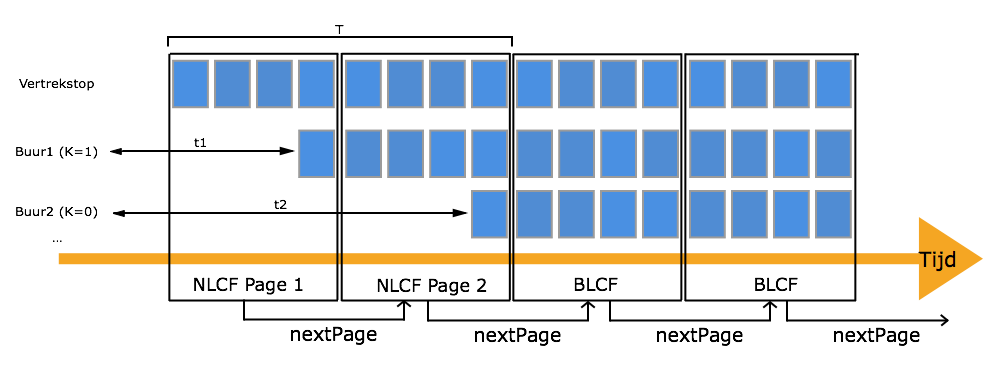
\includegraphics[scale=0.4]{OptimalisatieHypermedia}
\caption{Overzicht van resources van speed-up optimalisatietechniek.}
\label{OptimalisatieHypermedia}
\end{figure}

%Uit de resultaten \ref{dataverbruik-heuristiek} blijkt dat het eerste fragment bepaalt of het resultaat gevonden wordt of niet. Hierbij bevat het eerste fragment drie keer zoveel nuttige connecties.

\subsection{Hypermedia}

De originele implementatie maakt gebruik van hydra:nextPage links om volgende fragmenten te vinden. Dit principe kunnen we toepassen op een NLCF (zie ook \ref{OptimalisatieHypermedia}). Op deze manier kunnen we een grotere $T$ waarde instellen zonder dat kleinere routes onnodig veel connecties downloaden. $K$ moet maximaal zijn om te kunnen garanderen dat de optimale oplossingen ertussen zit.
Uit de resultaten van basic Linked Connections Fragments (zie \ref{fragmentgrootte}) blijkt dat queries gemiddeld het snelst opgelost zijn als de fragmenten een grootte hebben van rond de duizend connecties. Het initi\"ele NLCF wordt per duizend connecties onderverdeeld. Listing \ref{interface-met-hypermedia} toont de nieuwe interface. Het NLCF fragment bevat naast tijdsinterval $T$ ook een pagina-grootte. Hiervoor kan hetzelfde tijdsinterval genomen worden als basic LCF's.

\begin{lstlisting}[label=interface-optimalisatiemethypermedia,caption=Interface optimalisatie met hypermedia links]
http://example.org?departureTime={...}&departureStop={...}&page={...}
\end{lstlisting}
\label{interface-met-hypermedia}

Met deze techniek worden de twee nadelen (\ref{heuristiek-nadelen} van vorige techniek weggewerkt:
\begin{itemize}
\item Er is een hogere effici\"entie, omdat een groter tijdsinterval gekozen kan worden. Daarbij worden connecties slechts een keer teruggeven, omdat er slechts een NLCF gebruikt wordt.
\item De optimale oplossing wordt gevonden. De NLCF geeft een gefilterde lijst van connecties voor alle mogelijke buren (dankzij max $K$) terug die gesorteerd zijn volgens vertrektijd. Alle mogelijke connecties met vertrektijden binnen de query vertrektijd en $T$ worden beschouwd. Als de snelste route hierin ligt,  zal deze gevonden worden. Als de query nog niet gevonden is, wordt simpelweg verdergezocht met basic LCF's met vertrektijd na $T$. Deze garandeert ook een optimale oplossing.
\end{itemize}

%\subsection{Slimme cli\"ents}
%
%Uit de resultaten van de originele implementatie (\ref{}) blijkt dat er een lineaire afhankelijkheid is tussen afstand tussen start- en eindbestemming en de tijd nodig om de query op te lossen. Aangezien de cli\"ent weet wat de afstand is tussen start- en eindbestemming kan hij zelf beslissen om query's een bepaalde afstand enkel met een andere techniek op te lossen.  
%

